% Introduction of Tariff Generator Tool
\documentclass{beamer}
\usepackage{graphicx}
\usepackage{lipsum}

\begin{document}
\title{Tariff Generator Tool}   
\author{Krishna Paudel, Ivan Shubhashev} 
\institute{1\&1 Telecommunication}
\date{\today} 

\frame{\titlepage} 

%\frame{\frametitle{Table of contents}\tableofcontents} 

%%% INTRODUCTION %%%
\section{Introduction} 
\frame{\frametitle{Introduction} 
    \begin{itemize}
        \item This tool generates the tariff and setup information from the information stored in CSV file.
        \item Input of this tool is the CSV file and after processing, it generates two output files: \textit{tariff.xml} and \textit{setup.xml}
        \item The generated files are copied into the card module for shop. 
        \item The generation process gets information from the CSV file to generate the above-mentioned output files.
    \end{itemize}
}

\section{Motivation}
\frame{\frametitle{Motivation}
    \begin{itemize}
        \item Manually creating or editing tariff information has the chances of typos or human-errors.
        \item Automation generation simplifies the task of inserting the same information for multiple tariffs.
        \item By using plain CSV file, we can have the possibilities of traking the file in repositories (Git or Subversion)
        \item More scalable and maintainable.
    \end{itemize}
}


%%% BACKGROUND %%%
% tariff.xml file, setup.xml
\section{How it works?}
\frame{\frametitle{How it works?}
    \begin{itemize}
        \item The program takes the tariff information form the CSV file and creation XML content using this information.
        \item Before running the program, we have to be sure that all the tariffs are in the file. 
        \item The generation is carried out within seconds and if success, the output tariff files are created.
        \item If any problems, the cause of the problem is displayed, and can be corrected. (Mostly, bad file format, or input file does not exit)        
    \end{itemize}
}
\frame{\frametitle{Block diagram}
%Include a block diagram
}

\frame{\frametitle{Program Flow}
%Include a flow chart
}


%%% CONFIGURATION %%%
% CSV file info 
\section{File Structure}
\frame{\frametitle{CSV File}
%Include a CSV file 
}
\frame{\frametitle{CSV File Structure}
\begin{itemize}
    \item We need to be familiar with the CSV file structure to properly use this tool. 
    \item The columns represents the properties of the tariff
    \item Each row (except header rows) represent a tariff.
    \item \textbf{Note:} if active column is false, then the tariff is ignored by the tool. 
\end{itemize}
}


\frame{\frametitle{Colums of CSV file}
\begin{columns}
    \column{0.95\textwidth}
    \begin{description}
        \item[Title] Internal Name
        \item[BK Shop] BK-Shop
        \item[BK Shop - Umzug]Bk-Shop Umzug
        \item[UpT Aktion - Standard-Angebot] Standard UpT
        \item[UpT Aktion - Nk-Angebot/Sparpreistausch]  Sparpreistausch UpT
        \item[UpT Aktion - Retention Angebot]  Retention Angebot UpT
    \end{description}
        
    
\end{columns}
}



%%% PROGRAM STRUCTURE %%%
% Structure of the program, like the files and their significance
\section{Program Structure}
\begin{frame}
    \frametitle{Program Structure}
        \begin{itemize}
            \item 
        \end{itemize}   
\end{frame}


%%% TECHNICAL INFO %%%
% Python environment as docker environment
\section{Technology}
\frame{\frametitle{Technology Used}
    \begin{itemize}
        \item
    \end{itemize}
}

%%%RUNNING THE TOOL %%%
% Running methods
\section{Running}
\frame{\frametitle{How to Run?}
\begin{minipage}{0.5\textwidth}
    \begin{itemize}
        \item item 1
        \item item2
    \end{itemize}
\end{minipage}
}

%%% DEMO %%%
% Show the running of tool using different methods
\section{DEMO}
\frame{
    \frametitle{Demonstartion}
}

\section{Pictures}
\frame{\frametitle{Title}
    %\centering
    %    \begin{tabular}{c}
        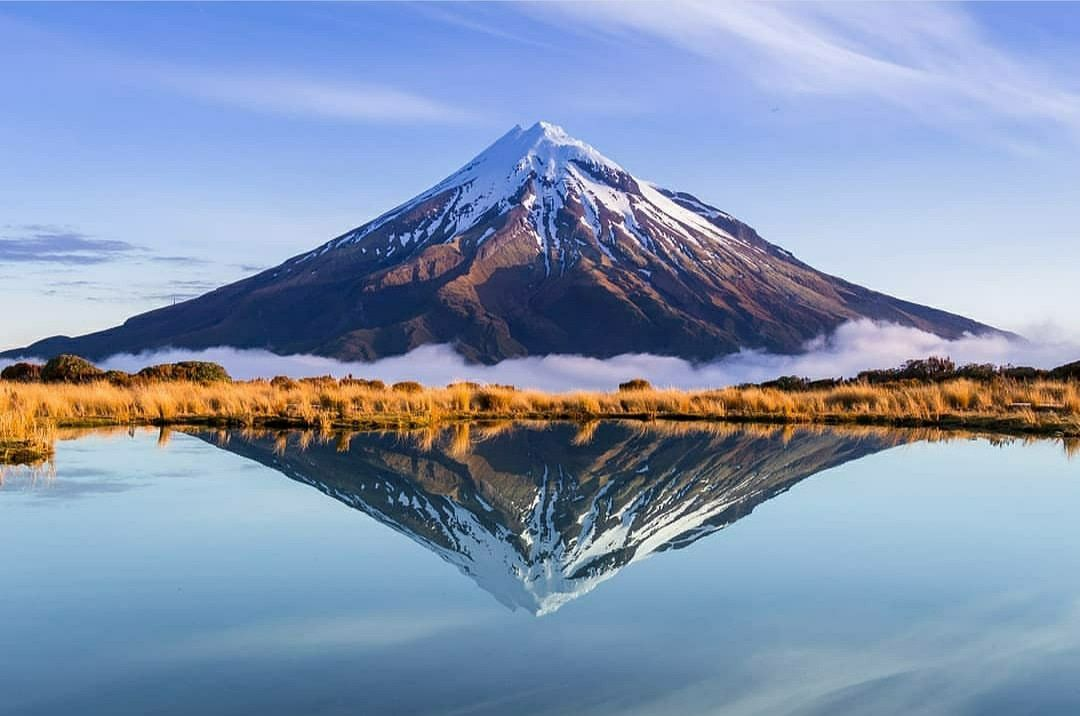
\includegraphics[width=0.9\linewidth,keepaspectratio]{images/pic.jpg}    
    %    \end{tabular}
}

\section{Conclusion}
\frame{\frametitle{Conclusion}
    THANK YOU!! \newline\newline

    Etwas fragen?


}
\end{document}

